\documentclass{article}

\usepackage[utf8]{inputenc}
\usepackage{graphicx} % Comandos para manejar imágenes
\graphicspath{ {./images/} } % Carpeta de imágenes

\setlength{\parskip}{2mm} % Espaciado

\usepackage[utf8]{inputenc}
\usepackage{geometry}
    \geometry{left=3cm,right=2cm,top=2cm,bottom=2cm}
%
\usepackage[spanish]{babel}
%
\usepackage[fixlanguage]{babelbib}
    \bibliographystyle{babunsrt}
%

\usepackage{floatrow}
\floatsetup[table]{style=plaintop}

\usepackage{url}

\usepackage[top=2cm, bottom=2.5cm, right=3 cm, left=3 cm]{geometry} % margenes

\usepackage{parskip} % Sangria

\title{Seminario tres: Modelando los negocios comentarios sobre la presentación de Doctor Guillermo Bustos}
\author{Cristóbal Galleguillos Ketterer$^{1}$\\
\small{$^{1}$Industrial PhD Program}\\
\small{Pontificia Universidad Católica de Valparaíso}\\
\small{cristobal.galleguillos@pucv.cl}
}
\date{\small{\today}}

\begin{document}

\maketitle

\section{Introducción}

Los procesos industriales (incluidos aquellos que podemos llamar comerciales o de servicios), están compuestos por una serie de sub procesos, los cuales, mediante el modelamiento cualitativo, permiten el análisis del negocio, de modo de permitir visualizar la complejidad de cada una de las tareas aisladas y la interdependencia de unas con respecto a las otras.

Sin duda, este es un procedimiento complejo, debido a la diversidad de organizaciones y a los distintos modelos funcionales que se desarrollan dentro de estas. La arquitectura de procesos de negocios (BPA, por sus siglas en inglés) es una herramienta que permite modelar los procesos de negocios y sus interrelaciones.

En este trabajo se hará una breve exposición de la presentación del Doctor Bustos, acerca de sus trabajos en esta materia, considerando su aporte la extensión del procedimiento BPA, por un método de arquitectura de procesos de negocios basado en el dominio (en conjunto con la Doctora (c) Ma. Fernanda Torres).


\subsection{Alcance}

El marco teórico se referirá en forma exclusiva a describir los aspectos basales de la presentación del Doctor Bustos. El lector encontrará más detalle en cualquier libro de modelo de proceso de negocios o de procesos industriales o de procesos de manufactura clásicos.

\section{Revisión de la literatura}

La producción científica en esta área es extensa, esto es una consecuencia directa de la diversidad de industrias y comercios que actúan en el mercado, los datos que aquí se presentan se basan en una selección de los 200 artículos más citados, desde la base de datos Scopus.

La Figura \ref{nube} representa el mapa de palabras mas comúnmente utilizadas en la investigación científica asociada ael estudio de los autores.

Un rápido vistazo puede dar cuenta de que este campo de investigación esta asociado a los procesos de manufactura y servicios modernos, siendo su penetración en la industria tradicional (ejemplo construcción, manufactura) menos corriente

\begin{figure}[H]
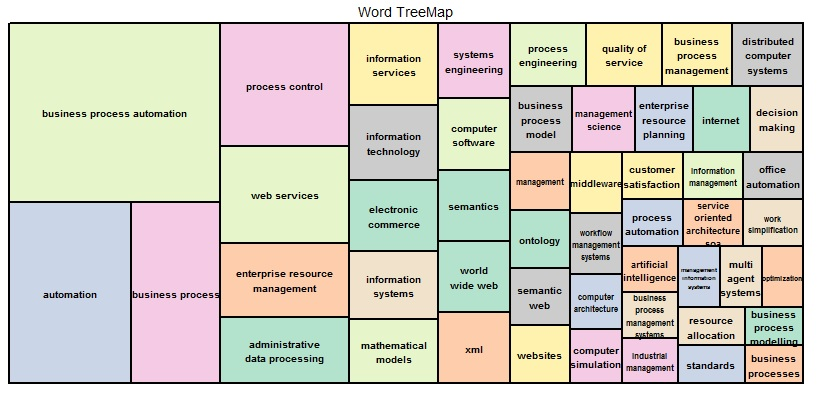
\includegraphics[scale=0.7]{Images/oTRO ARBOL.jpg}
\centering
\caption{Mapa de palabras}
\label{nube}
\end{figure}


La Figura \ref{arbolcon} presenta a la derecha los campos del conocimiento que interactúan y los autores originales y las citas, nuevamente llama la atención que los campos del conocimiento donde se aplican estos tópicos son relacionados a aspectos relativamente modernos de la investigación en ingeniería, como la minería de datos, la internet de las cosas, la industria 4.0, etc.



\begin{figure}[H]
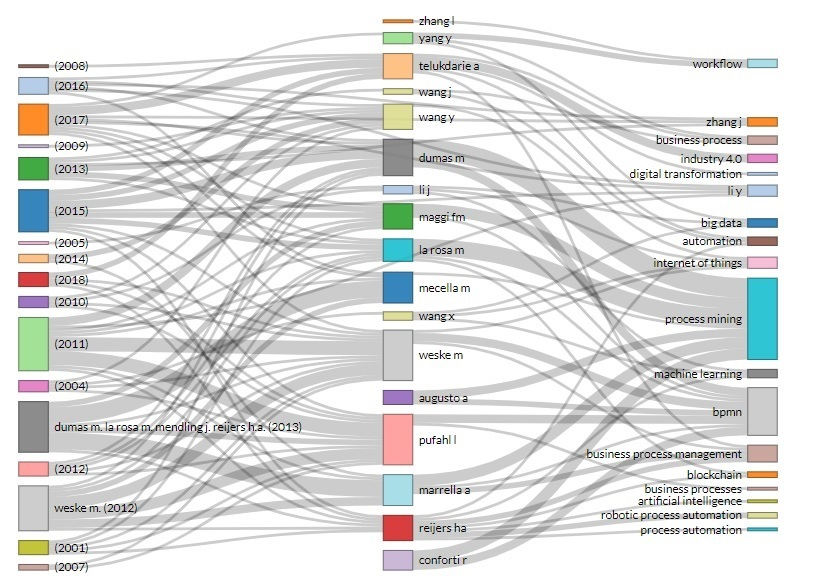
\includegraphics[scale=0.75]{Images/aRBOL.jpg}
\centering
\caption{Arbol de autores/citas/temas}
\label{arbolcon}
\end{figure}

La distribución de publicaciones por año se presenta en la Figura \ref{PCA}, existiendo un peak el año 2019.

\begin{figure}[H]
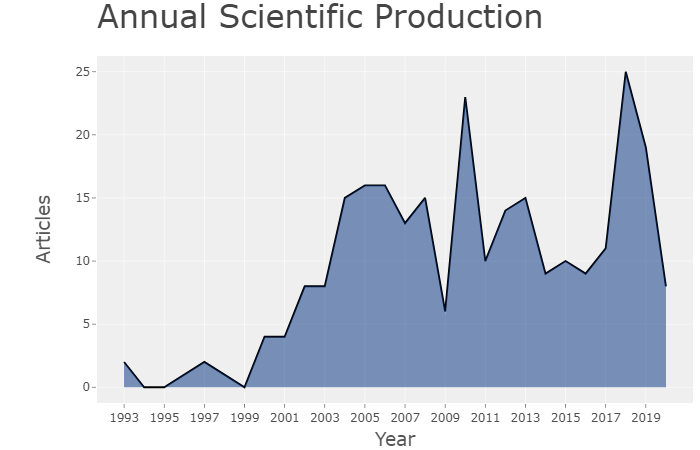
\includegraphics[scale=0.5]{Images/newplot (2).png}
\centering
\caption{Producción científica anual}
\label{PCA}
\end{figure}

Finalmente se presenta la producción por países, con clara predominancia de los países industrializados más China y Brasil (Figura \ref{mundoreal})

\begin{figure}[H]
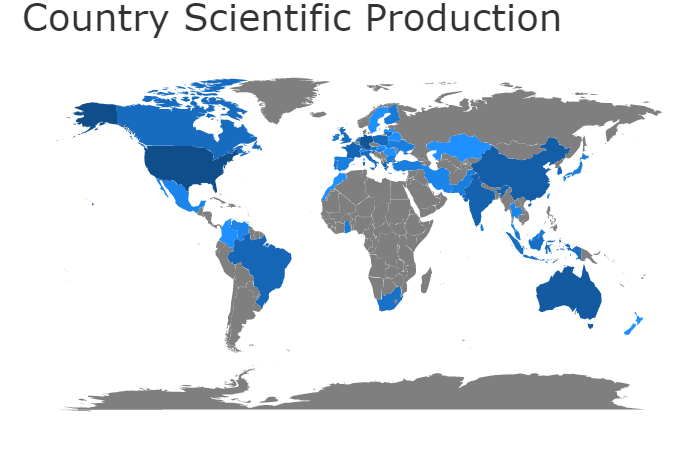
\includegraphics[scale=0.7]{Images/newplot (3).png}
\centering
\caption{Distribución de la producción científica en el mundo}
\label{mundoreal}
\end{figure}


\section{Marco teórico}

Un proceso de negocio puede descomponerse funcionalmente en tantos niveles de detalle como sea necesario. Los métodos de modelado generalmente prescriben dos o tres niveles de descomposición y uso de diferentes convenciones de nomenclatura para cada nivel (por ejemplo, proceso, actividad, tarea). 

Un buen punto de partida para el estudio de las arquitecturas de proceso de negocios, es considerar la norma internacional ISO 42010 \textit{Systems and software engineering — Architecture description} es un estándar internacional para la descripción de la arquitectura de sistemas y productos software.

En este cuerpo normativo se pretende normalizar y estandarizar la descripción de las arquitecturas considerando un lenguaje común y marcos de trabajo pre establecidos.

EL trabajo de \cite{art2:a2} presenta un interesante modelo de arquitectura basado en la norma ISO 42010, que se muestra en la Figura

\begin{figure}[H]
\includegraphics[scale=0.7]{Images/paper.jpg}
\centering
\caption{Main words \cite{art2:a2}}
\label{mundo}
\end{figure}


Los autores de \cite{art2:a2} definen las siguientes preguntas para reconocer un negocio posible de modelar mediante BPA.

\begin{enumerate}

\item¿Por qué? Un objetivo comercial es un objetivo que puede descomponerse. Cada objetivo puede estar asociado a los procesos comerciales que contribuyen a su logro. 

¿Dónde? Una unidad organizativa define la estructura organizativa. Puede describir una unidad lógica (por ejemplo un departamento) o una ubicación física o geográfica.

\item¿Cuando? Un cronograma comercial es un plan que especifica restricciones temporales para realizar procesos comerciales.

Por lo tanto, comprende los eventos que son importantes para la organización. Los horarios están vinculados a los procesos de negocio.

\item¿Qué? Una entidad de información representa la información sobre una persona, lugar, concepto, cosa o evento que tiene significado en el contexto de la empresa y sobre qué datos pueden almacenarse.

\item¿Quién? Un actor desempeña uno o más roles. Los actores pueden representar personas o sistemas, incluida la información sistemas y maquinas. Un actor puede desempeñar múltiples roles y el mismo papel puede ser desempeñado por diferentes actores.
 \end{enumerate}

\section{Contribución del autor}

El autor en su línea de investigación propone un cambio de enfoque, considera que los problemas modelados tradicionalmente (por ejemplo un ciclo de vida) no permiten ver más allá de la implementación, en este caso, el ciclo de vida es valioso para el cliente (\textbf{centrado en las actividades})

Adicionalmente, en el trabajo de la Doctora (c) González identificó tres problemáticas vinculadas a los métodos para el diseño de BNP \cite{lib1:T1}: 

\begin{enumerate}
\item Falta de insumos estructurados.
\item Consideración limitada de las relaciones entre procesos de negocio, y 
\item Uso restringido de lenguajes estándares de la industria.

 \end{enumerate}

La autora describe como la principal consecuencia de estos aspectos, a  la amenazan las métricas de calidad más relevantes de los métodos para el diseño de BPM, es decir, facilidad de uso y utilidad. 

Es por ello que los investigadores propone  un enfoque basado en entidades, identificando “que es” lo que se transforma en algo valioso. Este nuevo enfoque permite además modelar solo las actividades que generan valor.

A este enfoque se le llama método de APN basado en dominio (dPBA), \textbf{centrado en las entidades} (ver Figura \ref{enti})


\begin{figure}[H]
\includegraphics[scale=1]{Images/compara.jpg}
\centering
\caption{Cuadro comparativo distintos enfoques \cite{lib1:T1}}
\label{enti}
\end{figure}

Los autores, en el mismo contexto proponen pautas dinámicas de integración de modelos de negocios \cite{art1:a1}, en el ejemplo que se presenta a continuación después de ser puesta una orden, el pedido puede estar pendiente o confirmado dependiendo del Stock, y eventualmente se puede entregar (Ver Figura \ref{dinamico}). Esta es una parte de la línea de investigación de los autores que se produce por extensión de la anterior. 

\begin{figure}[H]
\includegraphics[scale=.7]{Images/2paperbusros.jpg}
\centering
\caption{Modelo dinámico \cite{art1:a1}}
\label{dinamico}
\end{figure}


\section{Comentarios}

\subsection{La empresa moderna, un sistema complejo }

La empresa moderna es un sistema complejo, es muy factible que las decisiones de marketing y diseño pueden estar en una oficina de Londres, las fábricas de insumos en india, las ensambladoras en China y el embalaje, almacenamiento y distribución en una ciudad de Estados Unidos.

En un caso así, serpia conveniente incluir en los flujos diversos procesos asociados a las legislaciones de cada país, incluyendo leyes sociales y ambientales y los riesgos asociados a los traslados.

Otro punto a considerar es la protección del producto, la alta dispersión fomenta la piratería, por lo que las entidades legales pueden llegar a tomar un rol relevante. 



\subsection{Marketing y toma de decisiones del cliente}

Es muy posible que los clientes no tomen decisiones racionales, por lo que las retroalimentaciones de estos no necesariamente influyan de forma positiva en las decisiones variables de las entidades, objetos como los de lujo, o que de algún modo generan un bienestar mayor al valor de uso y de cambio, puede sufrir dramáticos cambios en la demanda (ejemplo por perdida de reputación de una empresa) o bien en la producción (efectos de shock social causado por producción en países muy pobres con mano de obra muy barata) o bien cambios afectos a la materia prima (conciencia en el reciclaje, uso de áreas silvestres protegidas en las industrias, contaminantes, propiamente tal).

Este ambiente, puede generar dinamismos y cambios muy bruscos en los requerimientos del productor que eventualmente, debería el modelador considerar como una variable de decisión, que permita hacer cambios casi en tiempo real, en base a los recursos disponibles.

\subsection{Cultura organizacional versus procedimientos de trabajo}

Los modelos de producción, generalmente se basan en ideas preconcebidas de como las empresas deberían funcionar en su punto óptimo, en la mayoría de los casos, estos modelos procedimientos que rara vez se siguen y que no consideran la estructura organizacional, clásico es el ejemplo de implementación de ERP, que solamente se utilizan como registro mientras los procesos se realizan en las tradicionales plantillas Excel, una pregunta (a la cual no tengo respuesta), es como una arquitectura de sistemas empresariales podría evaluarse en función de cuan apegado está a la cultura organizacional y en base a ese modelo realizar los ajustes que optimicen los procesos.


\nocite{*}
    \bibliography{src/ref}

\end{document}
